\documentclass{standalone}
\usepackage{tikz}
\usepackage{ctex,siunitx}
\usepackage{tkz-euclide}
\usepackage{amsmath}
\usetikzlibrary{patterns, calc}
\usetikzlibrary {decorations.pathmorphing, decorations.pathreplacing, decorations.shapes,}
\begin{document}
\small
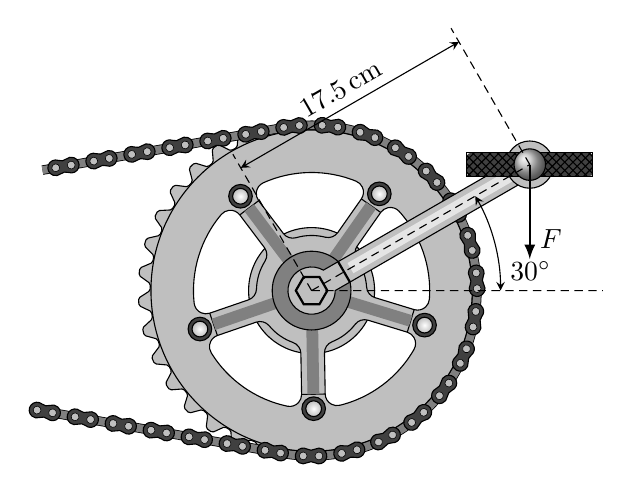
\begin{tikzpicture}[>=latex,scale=1.0]
  \draw[fill=lightgray](0,0)circle(0.8);
  \draw[fill=lightgray,rounded corners=0.2mm](110:2.05)--(112.5:2.2)arc(112.5:115:2.2)--(117.5:2.05)arc(117.5:120:2.05) 
  \foreach \x in{120,130,...,250}{--(\x+2.5:2.2)arc(\x+2.5:\x+5:2.2)--(\x+7.5:2.05)arc(\x+7.5:\x+10:2.05)}--(260:1.7)arc(260:110:1.7)--cycle
  ;
  \fill[lightgray,even odd rule,draw=black](0,0)circle(2.04)%(0,0)circle(1.5);
  \foreach \x in {55,127,...,360}
  {
    (\x+20.667:0.7)arc(\x-159.333:\x-90:0.15)--++(\x:0.5209)arc(\x-90:\x+12.84:0.15)arc(\x+12.84:\x+59.161:1.5)arc(\x+59.161:\x+162:0.15)--++(\x+252:0.5209)arc(\x-198:\x-128.667:0.15)arc(\x+51.333:\x+20.667:0.7)
  }
  ;
  \foreach \x in {55,127,...,360}
  {
    \draw(\x-6.501:1.325)--(\x+6.501:1.325);
    \draw[line width=1.5mm,gray](0,0)--(\x:1.316);
    \draw[fill=darkgray](\x:1.5)circle(0.15);
    \draw[outer color=lightgray,inner color=white](\x:1.5)circle(0.1);
  }
  \draw[fill=gray](0,0)circle(0.5);

  %% 链条
  \coordinate (A) at (100:2.1);
  \coordinate (B) at ([shift=(190:3.1)]A);
  \draw [
    line width=0.1mm,
    double=gray,
    double distance=1mm,
    postaction={decorate},
    decoration={
      markings,
      mark=between positions 0.02 and 1 step 4.9mm with 
      {
        \draw[thin, draw=black,fill=darkgray] ([shift=(60:0.1)]-0.1,0)arc(60:300:0.1)arc(120:60:0.1)arc(-120:120:0.1)arc(-60:-120:0.1);
        \draw[very thin,fill=lightgray](-0.1,0)circle(0.05);
        \draw[very thin,fill=lightgray](0.1,0)circle(0.05);
        } 
    }
  ] (B)--(A)arc(100:-100:2.1)--++(170:3.1);
  %% 脚踏
  \draw[fill=lightgray]([shift=(30:3.0)]60:0.3)--(60:0.3)arc(60:360:0.3)--++(30:3.0);
  \draw[thick](0:0.2)\foreach \x in {60,120,...,300}{--(\x:0.2)}--cycle;
  \draw[thick](48:0.5)--(12:0.5);
  \draw[line width=1.5mm,lightgray!40](30:0.57)--(30:3.2);
  \draw[fill=lightgray](30:3.2)circle(0.3);
  \fill[darkgray,rounded corners=0.5mm]([xshift=-0.8cm,yshift=-0.15cm]30:3.2)rectangle++(1.6,0.3);
  \draw[pattern=crosshatch]([xshift=-0.8cm,yshift=-0.15cm]30:3.2)rectangle++(1.6,0.3);
  \draw[ball color=lightgray](30:3.2)circle(0.2);
  \draw[thick,->](30:3.2)--++(0,-1.2)node[above right]{$F$};
  \draw[thin,densely dashed](0,0)--(3.7,0)(0,0)--(30:3.2)(0,0)--(120:2.0)(30:3.2)--++(120:2.0);
  \draw[thin,stealth-stealth] (2.4,0)arc(0:30:2.4)node[at start,above right]{\ang{30}};
  \draw[stealth-stealth](120:1.8)--++(30:3.2)node[midway,above,sloped]{\qty{17.5}{cm}};
\end{tikzpicture}
\end{document}